\chapter{Design}

This section will elaborate the design process with the client and modifications that occurred. The basic design was to start off with a transparent functional open source system and built upon that at every iteration. Having an ambitious project could result in client dissatisfaction if effort of project is underestimated.      

\section{Initial Design} 

After the initial meeting with the client, the system shown in figure \ref{intial-design} was designed with the following characteristics:

\begin{figure}[H]
  \centering
  \includegraphics[width=\textwidth]{initial_design}
  \caption{Initial Design}
  \label{intial-design}
\end{figure}

\begin{itemize}
  \item The team decided to use OM2M as the open source platform as it was developed by a well-known organization (The Eclipse Foundation produce the Eclipse IDE), uses a language the whole group were comfortable developing with (Java), and had a well-maintained repository with an active community that asks questions.
  \item As the project was about federating with the public deployed oneTRANSPORT platform, it was necessary to also have a publicly accessible server to achieve mutual communications. As Digital ocean offers a \$50 free credit for student via the GitHub education package it was decided to use Digital Ocean Droplet hosting for the OM2M IN-CSE. 
  \item The website for visualizing sensor data would also be hosted on the same droplet (with the use of sub domains, see section \ref{sec:web-services}). This web application would query the data via OM2M RESTful API. It will be written in PHP with Symphony as a web framework, as one team member had significant experience in this area.  
  \item A Raspberry Pi would act as the gateway holding the MN-CSE. Sensors would be attached to the PI via the GPIO pins.
  \item The Raspberry Pi would most likely be located on a NATed network, so it is crucial that a VPN tunnel is used to break out.
  \item Because the gateway(s) need to be directly accessible form the droplet server, the team decided to host a VPN server on a droplet connecting the MN-CSE to the IN-CSE though a private network. 
\end{itemize}

\section{Final Design}

The client suggested modifications to the initial design after the next meeting by removing or amending features of the project that they deemed as extras. They were looking for something that they could showcase at expositions, therefore were looking for portable sensors that could be used indoors. The team decided to use Raspberry Pi Sense HATs that connect directly to the GPIO pins to form a compact device with multiple sensors for measuring temperature, humidity and pressure.

The client was not interested in the website visualization for sensor data. InterDigital were more drawn towards the data federation between the deployed platform and their oneTRANSPORT system. They noted that if federation was successfully, oneTRANSPORT was linked to a Graphana visualization tool.

After modifications to the design, the final approach was divided into the following steps to organise development:

\subsection{Step 1: OM2M Development}

Developing and deploying the platform was the base step in this project. It involved requesting all the hardware necessary for deploying the IoT sensors and platform, developing the AE for gathering sensor data in Java and deploying the IN-CSE and MN-CSE on hardware (server and Raspberry Pi).

Figure \ref{development-design} shows the initially deployed platform running the Droplet server and gateway Raspberry Pi. OM2M uses by default a H2 database engine \cite{H22017H2Engine}. There is a VPN tunnel established between server and gateway used for mutual communications. Communications between the IN (server) and MN (Gateway) would be over the default HTTP POST and GET requests implemented in OM2M, as other options (CoAP or MQTT) required some amount of configuration.

\begin{figure}[H]
  \centering
  \includegraphics[width=.7\linewidth]{step1}
  \caption{Step 1 Development Design}
  \label{development-design}
\end{figure}

The Sensor Communications Scripts in figure \ref{development-design} were written in Python, as there were existing Python libraries for accessing the Raspberry Pi Sense HAT sensors. These scripts for gathering data, would be called from the OM2M Java AE. It was noted that there would be a performance issue with this approach (calling Python from Java) but optimising for efficiency was not a scope in this project.

\begin{figure}[H]
  \centering
  \includegraphics[width=.55\linewidth]{data_storage}
  \caption{OM2M Data Storage Design}
  \label{data-storage-design}
\end{figure}

As the Raspberry Pi is a light weight device that has constrained storage capabilities, figure \ref{data-storage-design} demonstrates the design decision to store all the sensor data on the cloud hosted IN-CSE. As seen on the figure \ref{data-storage-design}, the MN-CSE would run the Python scripts to get sensor data which would then be sent to the registered IN-CSE via the HTTP POST requests over the VPN tunnel. The INs CSE functions would store them to the H2 database. 

The final objective of this step was to set-up a public fully functional open source platform connected to the sensors. The goal was to pass relatively small data represented as a sequence single numbers (temperature, gyroscope and accelerometer data). The team would understand how sensor data is passed through the system and stored on the IN-CSE in container instances. As the server was publicly accessible, this enabled the team to federate the data with other public systems in future tasks.

\subsection{Step 2: OM2M to OM2M Federation}
\label{step2}

The next step involved investigating and experimenting how IN data federation would occur between two instances of the open source implementation. This involved duplicating the design in figure \ref{data-storage-design} to produce figure \ref{federation-research}.   

\begin{figure}[H]
  \centering
  \includegraphics[width=\textwidth]{om2m_fed}
  \caption{OM2M Federation Research}
  \label{federation-research}
\end{figure}

The second IN-CSEs was deployed on a second droplet server (identical to the first). The two Raspberry Pis (gateways of figure \ref{federation-research}) would each be connected to a respective IN-CSEs. Then the two IN-CSEs would register together. Both IN server should be able to read the data stored in the other IN. 

With the release of OpenMTC half way through this step the team decided to include interconnection of OM2M and OpenMTC to research how different service provider's platforms would react with each other. The server and gateway on the left side of figure \ref{federation-research} would have an MN and IN running the OM2M platform, while the right server and gateway would have a IN and MN implemented in OpenMTC. The main purpose of this would be researching into cross service provider communication before attempting it with oneTRANSPORT.  

\subsection{Step 3: OM2M to oneTRANSPORT Federation}
\label{step3}

Once InterDigital was shown how federation would work between two INs (inter and intra service provider mentioned in section \ref{step2}), the same techniques could be attempted federating with oneTRANSPORT.

\begin{figure}[H]
  \centering
  \includegraphics[width=\textwidth]{step2}
  \caption{Step 2 Federation to oneTRANSPORT}
  \label{federation-to-ontransport}
\end{figure}

As seen in figure \ref{federation-to-ontransport}, without any prior technical knowledge of oneTRANSPORT, the team could interconnect open source platforms to InterDigitals platform via the same techniques mentioned in the previous section. This is dependent on an important assumption, that the two platforms have been correctly implemented using the oneM2M standard. OneTRANSPORT's IN and MN can be seen on the right side of figure \ref{federation-to-ontransport} and figure \ref{use-onetransport-grafana}.
\begin{figure}[H]
  \centering
  \includegraphics[width=\textwidth]{step3}
  \caption{Step 3 Use oneTRANSPORT Grafana}
  \label{use-onetransport-grafana}
\end{figure}

If data federation is successful, InterDigital could use their Grafana \cite{Grafana2018GrafanaMonitoring} engine to visualize the data originating from the In-CSE. As seen in figure \ref{use-onetransport-grafana}, oneTRANSPORT's IN-CSE contains an AE that will write all incoming data to Graphite \cite{Graphite2018Graphite} database, specialised in storing time series data. Grafana web visualisation tool will use the time series data to display metrics and analytics to the user.

\subsection{Camera Streaming}
\label{stream}

To tests the limits of the potential data being passed through the open source oneM2M platforms, the Raspberry Pi camera was used to produce image frames to be saved on the IN. A series of image data was launched, providing the IN with the maximum possible of images per second forming a video stream. OneM2M architecture specifies the rolling data base functionality, that is implemented in OM2M and OpenMTC. This would make sure that the size of the H2 database never significant grows by only keeping the most recent frames. The image data would be accessible from the INs RESTful API that will be used to display the video stream to end users.

\subsection{OM2M and OpenMTC}

Midway through November, a newly open sourced oneM2M platform (OpenMTC) written in Python was discovered. As the sensor scripts were written in Python, it would be easy to implement the exact same design mentioned in sections \ref{step2} and \ref{step3} but with OpenMTC platform over OM2M. The goal would be to compare efficiency and scalability with OM2M and OpenMTC in terms of data federation and data streaming (from section \ref{stream}). This also provided a mitigation against one project risk, without access to oneTRANSPORT, federation could still be demonstrated between two open source service providers (OM2M and OpenMTC).

\section{Raspberry Pi Scripts}

Due to shear complexity, it is undesirable to interact with the Sense HAT directly. Instead a program can write a Python script to take advantage of the \lstinline{sense-hat} library \cite{RaspberryPiFoundation2017SenseHAT}. This convenient library abstracts away direct i2c and GPIO communication into easy to use Python classes. From here, many individual Python scripts were written to initialise a specific sensor, read a value, and output the result as CSV (Comma Separated Values). This output would then be read by the platform, and stored in it's database.

\subsection{List of Python Scripts}

Below is a comprehensive listing of the Python scripts used in this project. Each of them is responsible for interacting with a unique sensor, be it on the Sense HAT or on the Raspberry Pi itself.\\

\begin{lstlisting}[caption={List of Python scripts}, label={lst:sensor-scripts}]
accelerometer.py, blink.py, camera.py, clear.py, compass.py, cpu.py, disk.py, gyroscope.py, humidity.py, icons, lowlight.py, memory.py, null.py, one.py, orientation.py, pixels.py, pressure.py, process.py, quality.py, rand.py, rotation.py, scroll.py, temperature.py, time.py, uptime.py, wifi.py, zero.py.
\end{lstlisting}

\subsection{Streaming Data}

Streaming was accomplished by adapting the previously mentioned Python scripts to run inside of a simple framework. This framework would check \lstinline{argv} and if a number was passed as the first parameter, it would be treated as the delay. So, for example \lstinline{./temperature.py 0.1} would respond with the current temperature every 0.1 seconds, or 10 times a second. If this number wasn't passed, then only one value would be returned before the script exited. With this approach, a plug-in can trivially support both single data points, along with streams of data.

\subsection{Daemon Script}

Additionally, a small daemon scripts was created to help manage and configure the Raspberry Pi. It runs at start up, and has two main tasks:

\begin{itemize}
\item Gather information about the status of the Raspberry Pi and display it on the 8$\times$8 LED matrix.
\item Allow the user to interact with the joystick removing the need to connect the Raspberry Pi to an external monitor to understand what technical issues may be happening.
\end{itemize}

A task of pinging the VPN server was created:\\

\begin{lstlisting}
ping IN-CSE-VPN-SERVER
\end{lstlisting}

This command would send an ICMP request packet to the IN-CSE VPN server IP address to verify that there is a valid VPN connection between the Raspberry Pi and the server. If the \lstinline{ping} is successful, the server will reply with a ICMP reply packet and the Raspberry Pi would display the time taken for this reply.   

Checking the status between the MN (Running on the Raspberry Pi) and IN (Web hosted server) was achieved by scheduling the task above, every 10 seconds. Light designs for the three states were defined (Can be seen in \ref{fig:led-matrix-status-images}):

\begin{itemize}
\item \textbf{Status OK}: Represented as a green OK in figure \ref{fig:led-matrix-status-images}). The \lstinline{ping} successfully replies letting the user know that the VPN is correctly functioning.
\item \textbf{Status Pending}: Represented by the grey question mark in figure \ref{fig:led-matrix-status-images}. This means the \lstinline{ping} request to the VPN is pending (waiting for a reply).
\item \textbf{Status Failed}: Represented by the red exclamation mark in figure \ref{fig:led-matrix-status-images}). This means the \lstinline{ping} request to the VPN server as failed (time-out).
\end{itemize}

In the case where the VPN connection would unexceptionally drop between the MN and IN, making communication from IN to MN impossible, the user would have a quick visual notification indicating the issue.   

\begin{table}[H]
\centering
\begin{tabular}{l|l|l}
\includegraphics[scale=0.9]{ok}&\includegraphics[scale=0.9]{unknown}&\includegraphics[scale=0.9]{warning_red}\\
\end{tabular}
\caption{LED Matrix Status Images}
\label{fig:led-matrix-status-images}
\end{table}

Due to the low resolution of the LED matrix, pixel art was employed to ensure that the meaning of resulting image was clear to the end user. As shown in figure \ref{fig:led-matrix-status-photos}, the image is clear in easily deciphered due to the coloured border, and the bright white icon. Originally, a single pixel was used to indicate VPN status, but this was quickly changed to help clarify the signal, and to provide redundancy in case of LED failure.

\begin{table}[H]
\centering
\begin{tabular}{l|l|l}
\includegraphics[width=0.305\textwidth]{okpicture}&\includegraphics[width=0.305\textwidth]{unknownpicture}&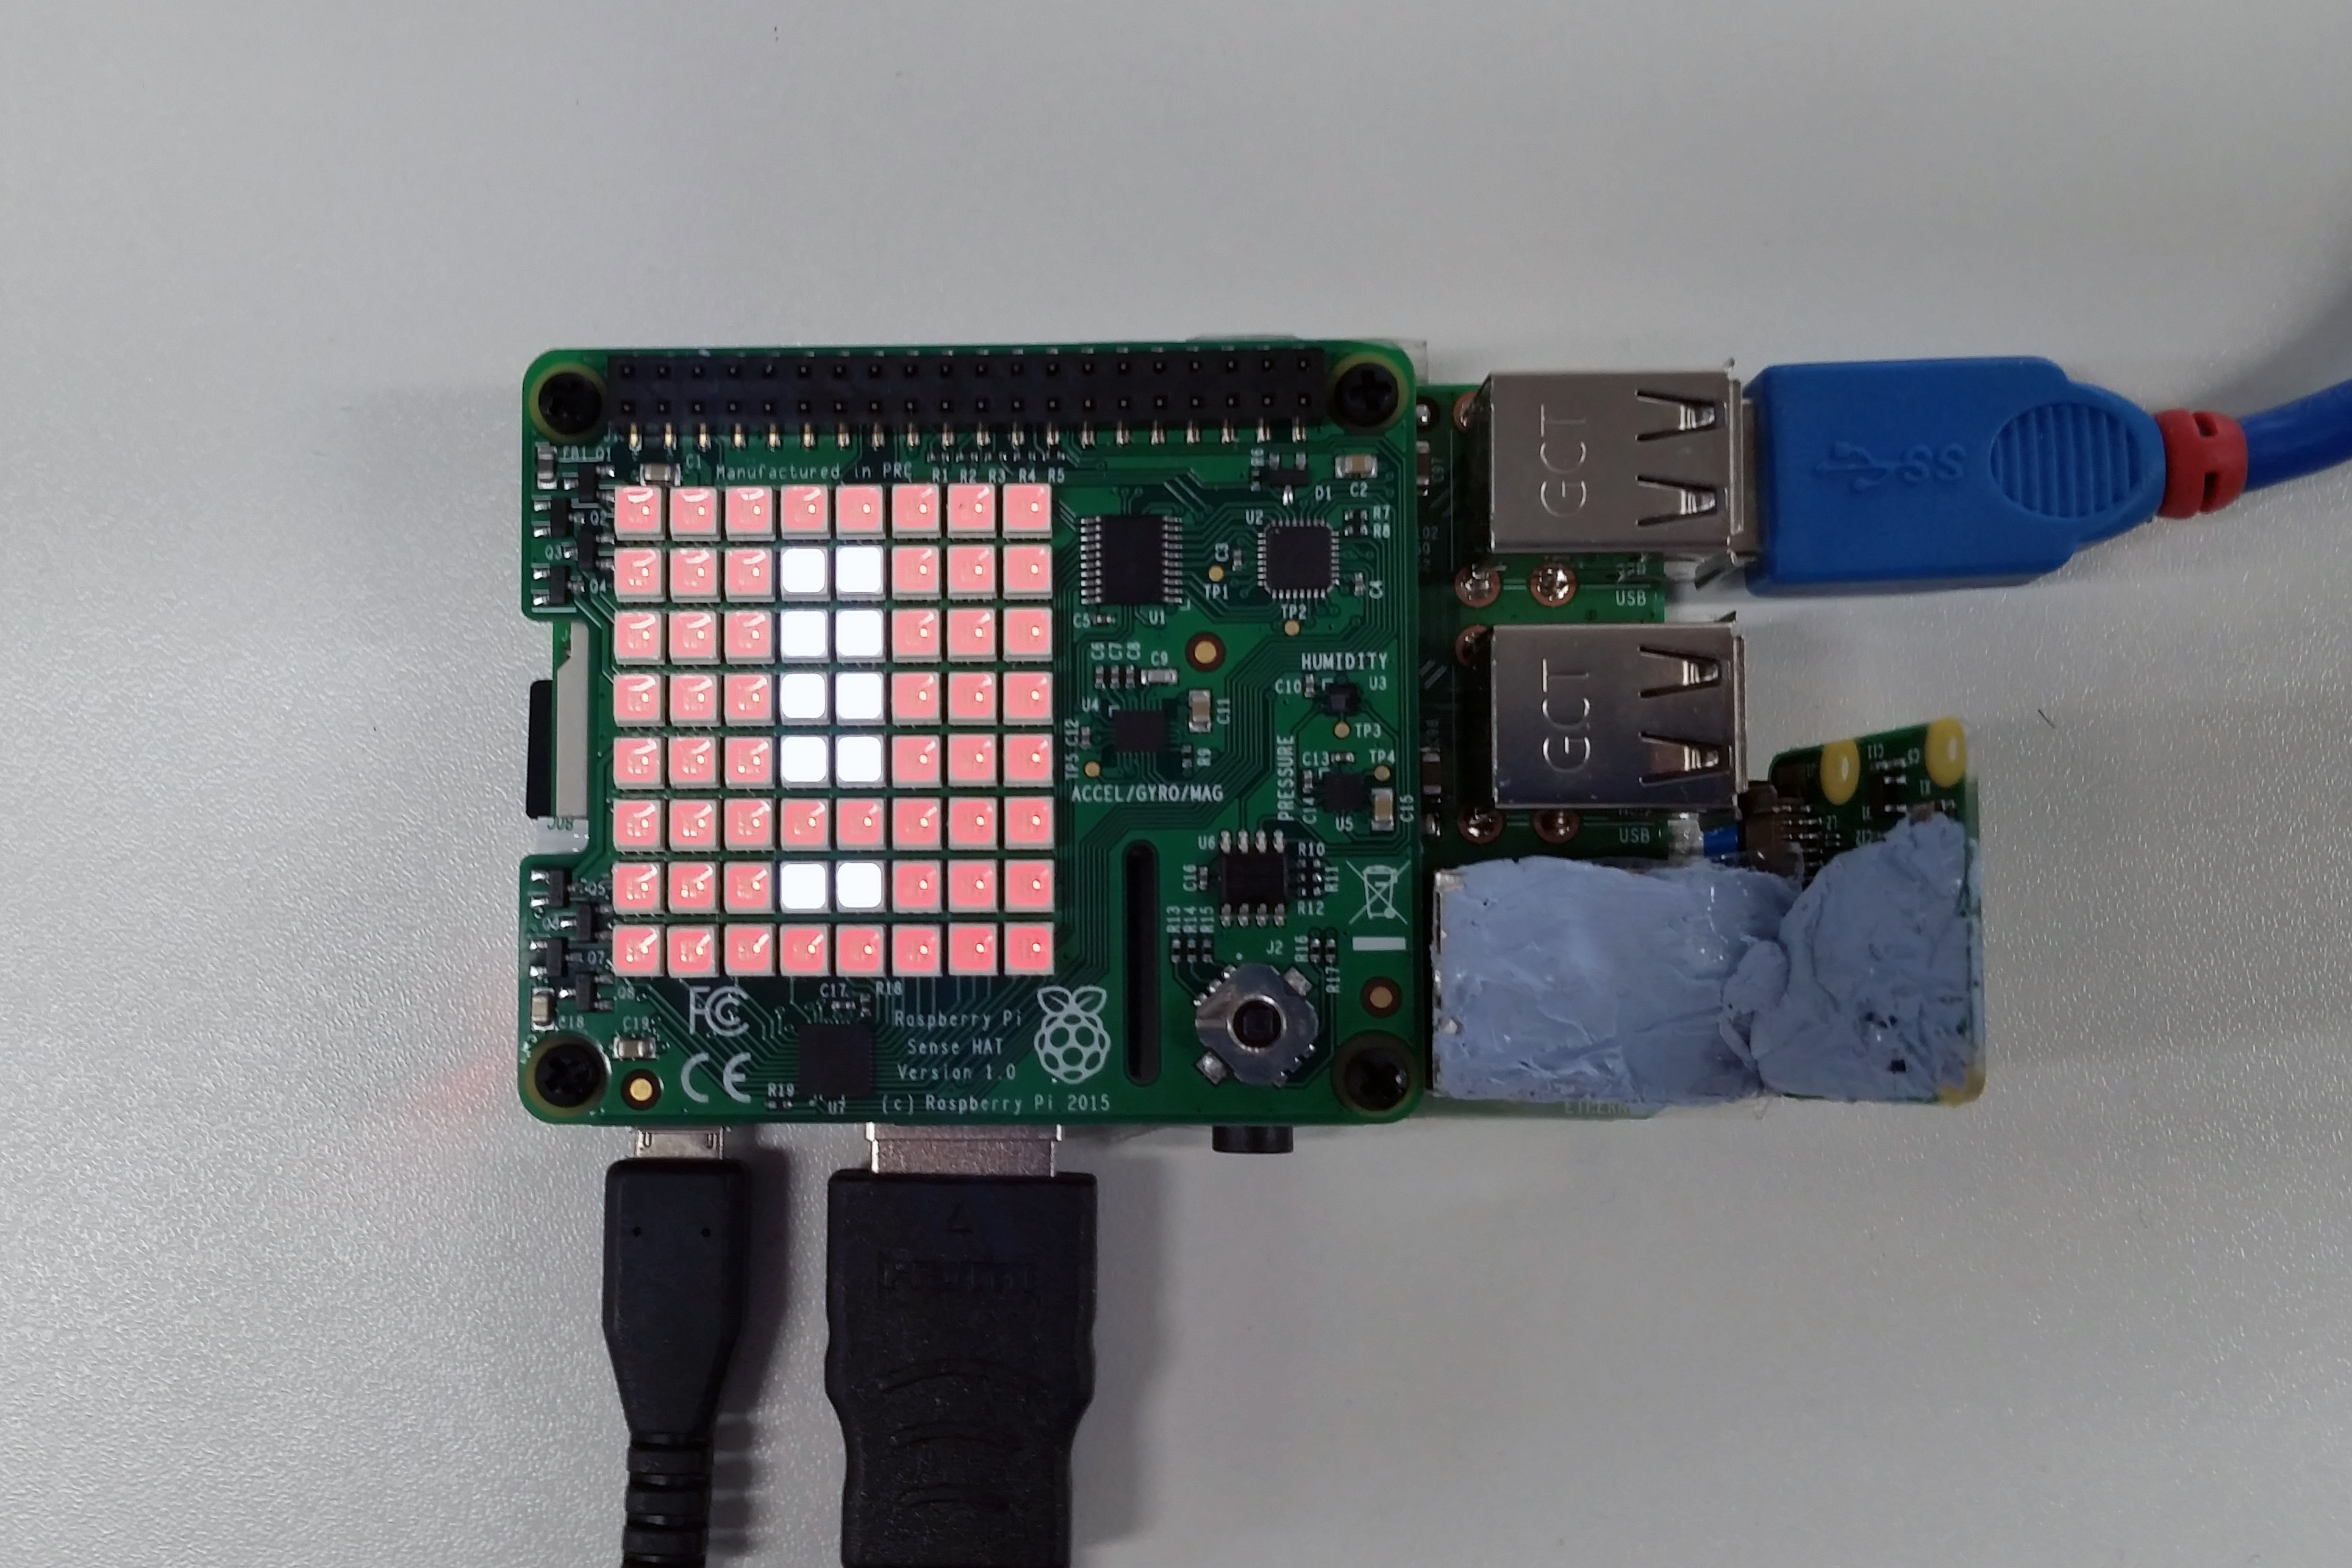
\includegraphics[width=0.305\textwidth]{errorpicture}\\
\end{tabular}
\caption{LED Matrix Status Photos}
\label{fig:led-matrix-status-photos}
\end{table}

Additionally, by pressing down on the joystick a user could either safely shut down the Raspberry Pi or reboot it. This functionality was added to help protect the integrity of the file system from unexpected power loss. As the device is designed to function automatically and without user interaction once powered, it is unlikely to have a keyboard or screen attached. Therefore, the user needs a simple method to quickly power off the device. Without such functionality, the user would likely simply remove power to the device, which has the potential of corrupting and destroying the file system, rendering the device unbootable until re-flashed.

\subsection{Automatically Running on Boot}

What is the point of a daemon script that doesn't run on boot? Nothing. That's why \lstinline{daemon.py}, OpenVPN, and either OpenMTC or OM2M (Depending on the build) are configured to run automatically on boot. This is achieved by proper configuration, and by using Linux \lstinline{/etc/init.d} scripts. Once installed, these scripts provide \lstinline{restart}, \lstinline{start}, \lstinline{status}, and \lstinline{stop} actions. Below is an example header:\\

\begin{lstlisting}[caption={init.d Header}, label={lst:header}]
#!/bin/sh
### BEGIN INIT INFO
# Provides:          SERVICE-NAME
# Required-Start:    $remote_fs $syslog
# Required-Stop:     $remote_fs $syslog
# Default-Start:     2 3 4 5
# Default-Stop:      0 1 6
# Short-Description: Start daemon at boot time
# Description:       Enable service provided by daemon.
### END INIT INFO

...
\end{lstlisting}

By adjusting the header, the name, description, order, and dependencies of a service can all be chosen. It is a flexible format, and what cannot be done in the header, can be done in the Bash script.

\subsubsection{Installing an init.d script}

\begin{enumerate}
\item Create a \lstinline{init.d} script from a template in \lstinline{/etc/init.d}.
\item Mark it executable with \lstinline{chmod +x /etc/init.d/$SERVICE-NAME}.
\item Install the init script with \lstinline{sudo update-rc.d $SERVICE-NAME defaults && sudo update-rc.d $SERVICE-NAME enable}.
\item Reboot the system, and service will run automatically.
\end{enumerate}

\subsection{Automatically Starting OpenVPN}

By default, OpenVPN will not automatically start, and will require the user to manually configure it after every boot. This can be fixed with the following two commands, assuming that \lstinline{config.ovpn} and \lstinline{certificate.crt} exist in the current directory.\\

\begin{lstlisting}[caption={Configuring OpenVPN}, label={lst:configuring-openvpn}]
sed -i -r 's/#AUTOSTART="all"/AUTOSTART="all"/g' /etc/default/openvpn
openvpn --client --config config.ovpn --daemon
\end{lstlisting}

The first line uncomments the \lstinline{AUTOSTART} variable in \lstinline{/etc/default/openvpn} so that when OpenVPN is started as a daemon (Runs in the background), on next boot it will start automatically.

\subsection{Building an image}

Once the Raspberry Pi was considered good and fully functional, an image was made. This was done by shutting down the Raspberry Pi to avoid damaging the file system, removing the microSD card, and inserting it into a computer to be read. Then, the device is mounted, and backed up using the following command:\\

\begin{lstlisting}[caption={Creating an image}, label={lst:backup}]
dd if=/dev/sdX conv=sync,noerror bs=64K | gzip -c > backup.img.gz
\end{lstlisting}

Then, to write the image to additional microSD cards, use the following command:\\

\begin{lstlisting}[caption={Restoring an image}, label={lst:restore}]
gunzip -c backup.img.gz | dd of=/dev/sdX
\end{lstlisting}

Now either the image, or microSD cards can now be shared. Due to how \lstinline{dd} creates disk images, images can only be flashed onto microSD cards with at least as much storage as the original microSD card. To resolve this issue, disk images can be shrunk using \lstinline{parted} or GParted.

\clearpage
